\begin{center} \LARGE \bf Ficha Catalográfica \end{center}


\begin{enumerate}
    \item Estas instruções \textbf{não} devem ser entregues aos avaliadores do trabalho nas ocasiões dos TCCs 1 e 2. Portanto, comente a linha que importa este arquivo;
    \item A ficha catalográfica deve ser elaborada após a defesa do TCC2, quando você concluir as correções sugeridas pela banca e validar a versão final com o/a professor(a) orientador(a);
    \item Acessar \url{http://repositorioinstitucional.uea.edu.br:8080/ficha/ficha_catalografica.php} e preencher as informações requeridas para elaborar a ficha catalográfica;
    \item Incluir o pdf gerado na subpasta \emph{source} com o nome \texttt{ficha.pdf};
    \item Apagar todo o conteúdo deste arquivo e deixar apenas o comando a seguir:
    \begin{verbatim}
        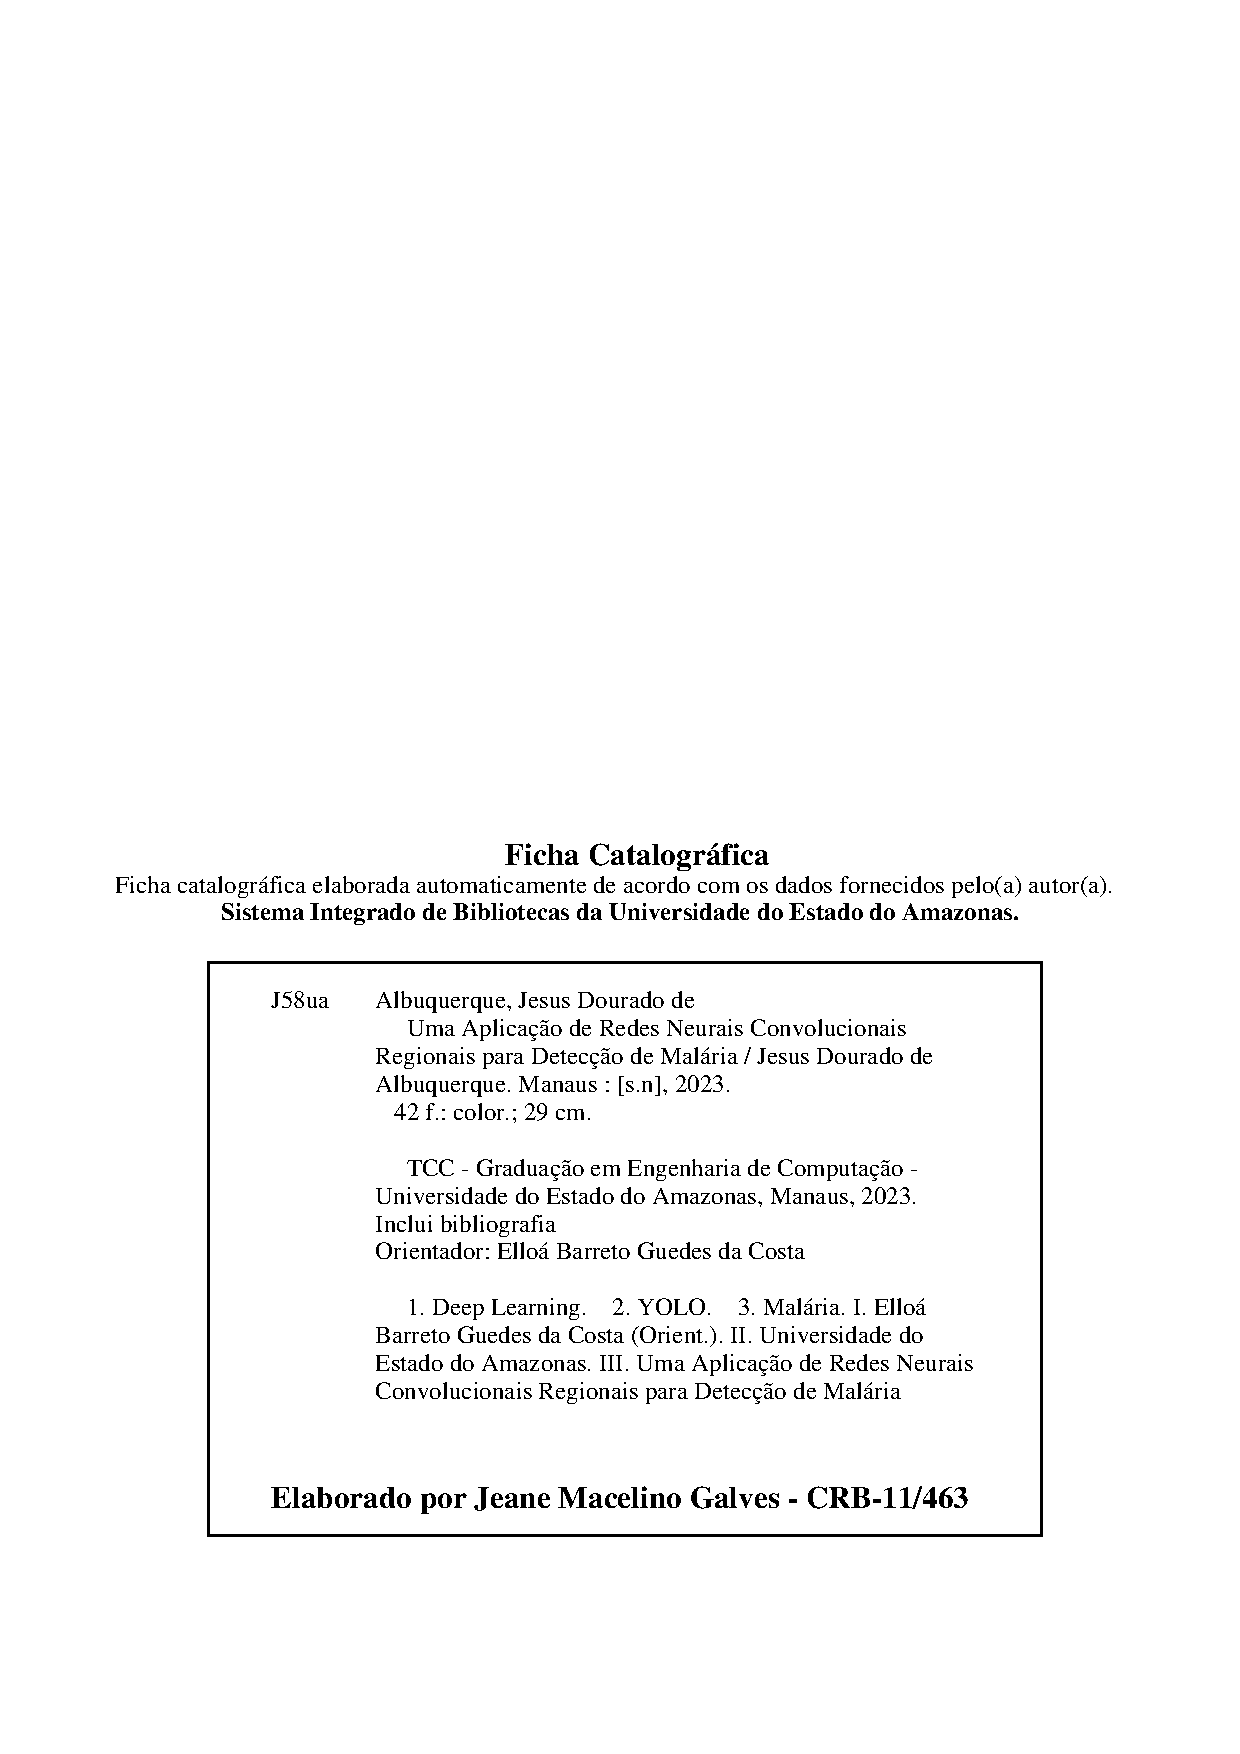
\includepdf[pages=-]{./source/ficha.pdf}
    \end{verbatim}
\end{enumerate}

\newpage
